% ICASSP 2027 pre-results manuscript.
% The official ICASSP 2027 author kit is not yet available; this draft uses
% the official ICASSP 2026 spconf package as a temporary layout scaffold.
\pdfminorversion=7
\pdfinfoomitdate=1
\pdfsuppressptexinfo=15
\documentclass{article}

\usepackage{vendor/icassp2026/spconf}
\usepackage{amsmath}
\usepackage{amssymb}
\usepackage{booktabs}
\usepackage{graphicx}
\usepackage{microtype}
\usepackage{multirow}
\usepackage{pifont}
\usepackage{xcolor}
\usepackage{xspace}

\definecolor{DraftRed}{HTML}{A50F15}
\definecolor{DraftFill}{HTML}{FEE5D9}
\definecolor{MethodBlue}{HTML}{0072B2}
\definecolor{MethodOrange}{HTML}{E69F00}
\definecolor{MethodGreen}{HTML}{009E73}

\definecolor{cvprblue}{rgb}{0.21,0.49,0.74}
\usepackage[pagebackref,breaklinks,colorlinks,allcolors=cvprblue]{hyperref}

\newif\ifsubmission
\ifdefined\RACsubmission
  \submissiontrue
\else
  \submissionfalse
\fi

\newcommand{\draftbanner}{%
  \ifsubmission\else
    \begin{center}
      \fcolorbox{DraftRed}{DraftFill}{%
        \parbox{0.92\columnwidth}{\centering\bfseries\color{DraftRed}
        DRAFT --- RESULTS PENDING}}
    \end{center}
  \fi}

\makeatletter
\newcommand{\DeclareResult}[2]{%
  \expandafter\gdef\csname rac@result@#1\endcsname{#2}}
\newcommand{\DeclareProtocolField}[2]{%
  \expandafter\gdef\csname rac@protocol@#1\endcsname{#2}}
\newcommand{\DeclareResultClaim}[2]{%
  \expandafter\gdef\csname rac@claim@#1\endcsname{#2}}
\newcommand{\DeclareAbstractResult}[1]{\gdef\rac@abstractresult{#1}}

\newcommand{\R}[1]{%
  \@ifundefined{rac@result@#1}{%
    \ifsubmission
      \PackageError{rac-paper}{Missing audited result `#1'}%
        {Populate generated/evidence_values.tex only after all result audits.}%
    \else
      \textcolor{DraftRed}{\scriptsize\textsc{pending}}%
    \fi
  }{\csname rac@result@#1\endcsname}}

\newcommand{\Protocol}[1]{%
  \@ifundefined{rac@protocol@#1}{%
    \ifsubmission
      \PackageError{rac-paper}{Missing verified protocol field `#1'}%
        {Bind this field to the frozen artifact manifest.}%
    \else
      \textcolor{DraftRed}{\textsc{pending}}%
    \fi
  }{\csname rac@protocol@#1\endcsname}}

\newcommand{\C}[1]{%
  \@ifundefined{rac@claim@#1}{%
    \ifsubmission
      \PackageError{rac-paper}{Missing audited result claim `#1'}%
        {Run result-to-claim and paper-claim audits first.}%
    \else
      \textcolor{DraftRed}{\textsc{Result-dependent statement withheld.}}%
    \fi
  }{\csname rac@claim@#1\endcsname}}

\newcommand{\ControlledAbstractResult}{%
  \@ifundefined{rac@abstractresult}{%
    \ifsubmission
      \PackageError{rac-paper}{Missing audited abstract result sentence}%
        {Declare exactly one sentence in generated/evidence_values.tex.}%
    \else
      \textcolor{DraftRed}{Experimental evidence is pending synchronization
      with the collaborator's frozen implementation and audited MultiRep runs.}%
    \fi
  }{\rac@abstractresult}}
\makeatother

\InputIfFileExists{generated/evidence_values.tex}{}{}

\newcommand{\method}{our proposed counter\xspace}
\newcommand{\checkmarkcell}{\ding{51}}
\newcommand{\xmarkcell}{\ding{55}}
\newcommand{\ClaimMap}[1]{}

\setlength{\abovecaptionskip}{4pt}
\setlength{\belowcaptionskip}{-2pt}

\newcommand{\bX}{\mathbf{X}}
\newcommand{\bZ}{\mathbf{Z}}
\newcommand{\bc}{\mathbf{c}}
\newcommand{\bm}{\mathbf{m}}
\newcommand{\bg}{\mathbf{g}}
\newcommand{\bq}{\mathbf{q}}
\newcommand{\cK}{\mathcal{K}}
\newcommand{\cL}{\mathcal{L}}
\newcommand{\cP}{\mathcal{P}}
\newcommand{\cD}{\mathcal{D}}
\DeclareMathOperator*{\argmaxop}{arg\,max}

% Author information explicitly approved for the single-anonymous draft.
% The complete collaborator roster and submission attestations remain gated.
\def\RACKnownAuthorNames{Weiping Yan}
\def\RACKnownAuthorAffiliations{University of Minnesota Twin Cities}
\def\RACKnownAuthorEmails{yan00944@umn.edu}

% Active ICASSP figure include. The legacy framework.* and task_comparison.*
% assets are retained for provenance but are retired from this include file.
\begin{figure*}[t]
  \centering
  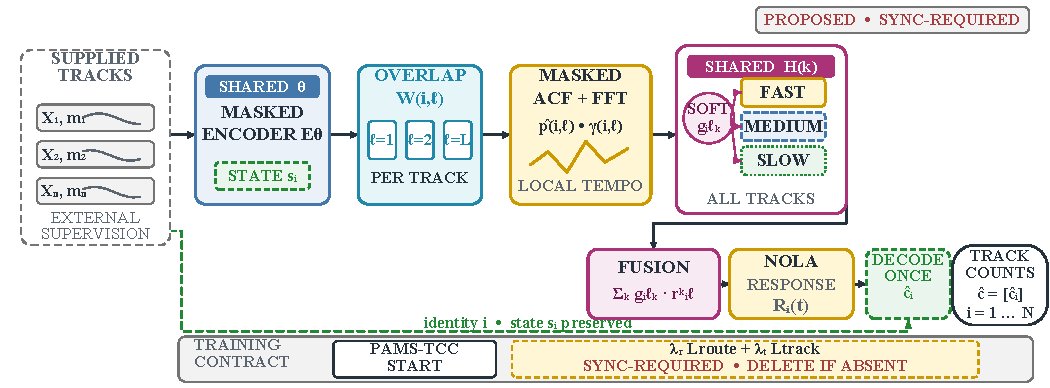
\includegraphics[width=\textwidth]{figures/icassp_framework.pdf}
  \caption{Proposed, synchronization-pending counting specification; this
  diagram is not implementation or result evidence. Supplied pose tracks and
  masks lie outside the counting boundary. The encoder and fast/medium/slow
  experts share parameters across identities, whereas dashed green elements
  carry identity-indexed state. Window-local masked ACF/FFT evidence drives
  soft routing; responses are fused, combined by normalized overlap-add, and
  decoded once per track. Training terms marked \texttt{SYNC-REQUIRED} remain
  explicit placeholders until the collaborator implementation is frozen.}
  \label{fig:icassp-framework}
\end{figure*}


\title{TempoRAC: Identity-Indexed Local Tempo Routing for Multi-Person Repetition Counting}

% ICASSP uses single-anonymous review. The draft shows the author identity
% explicitly approved by the user. Submission mode still receives the complete,
% assented roster through ignored private metadata after external validation.
\ifsubmission
  \ifdefined\RACAuthorNames
    \name{\RACAuthorNames}
    \address{\RACAuthorAffiliations\\\RACAuthorEmails}
  \else
    \name{\RACKnownAuthorNames}
    \address{\RACKnownAuthorAffiliations\\\RACKnownAuthorEmails}
  \fi
\else
  \name{\RACKnownAuthorNames}
  \address{\RACKnownAuthorAffiliations\\\RACKnownAuthorEmails}
\fi

\begin{document}
\ninept
\maketitle
\draftbanner

\begin{abstract}
\begin{abstract}
\draftbanner
Multi-person repetitive action counting (MRAC) must assign repetitions to
the correct person even when several people act asynchronously and each
person accelerates, decelerates, pauses, or disappears behind an occluder.
The MultiCounter family jointly learns detection, association, and counting
from annotated RGB videos, while label-efficient pose counters are
primarily developed for a single dominant actor. We study the complementary
setting in which a counting model receives identity-indexed pose tracks but
uses no person-wise count or period annotation during its intended counting
training. Our proposed design shares one pose encoder and a bank of tempo
experts across people while keeping temporal state separate for every
identity. Within overlapping windows, masked period evidence drives a soft
fast--medium--slow router. Expert responses are fused by normalized
overlap-add, after which each identity is decoded once, removing the direct
arithmetic double-counting path created by summing independent windows. The
primary output is a
person-wise count vector rather than only a scene total. \ControlledAbstractResult{} The
current manuscript is an evidence-gated pre-results specification: exact
auxiliary losses, frontend choices, and every empirical statement remain
blocked until they are reconciled with frozen code and machine-readable
artifacts.
\end{abstract}

\end{abstract}

\begin{keywords}
repetition counting, multi-person signals, local tempo, pose trajectories,
temporal routing
\end{keywords}

\section{Introduction}
\label{sec:introduction}

Repetitive motion is a useful measurement primitive. Exercise coaching,
rehabilitation, industrial monitoring, sports analysis, and human--robot
interaction all require more than recognizing that an action repeats: a
system must determine how often each participant repeats it. In an
uncontrolled scene, however, people need not move together. One person may
slow down while another accelerates, a third may pause, and tracks may contain
gaps caused by occlusion. A single response curve for the whole frame can
therefore mix identities and incompatible time scales, producing a plausible
scene total while assigning the wrong count to each person.

Repetition counting has progressed from online local cycle
estimation~\cite{levy2015live} and motion-frequency
analysis~\cite{runia2018realworld} to learned
temporal self-similarity, density regression, and dynamic-query models
~\cite{dwibedi2020repnet,hu2022transrac,ma2026detrc}. ESCounts studies
exemplar-conditioned counting and predicts one target density/count stream
~\cite{sinha2024escounts}. SkimFocusNet studies exemplar-selected multiple
action types~\cite{zhao2025skimfocus}. These advances largely assume one
counted stream. MultiCounter formalizes multi-instance repetitive action
counting and jointly predicts people, identities, periodic intervals, and
counts~\cite{tang2024multicounter}; MultiCounter+ strengthens temporal identity
consistency and long/short-period awareness~\cite{tang2026multicounterplus}.
Consequently, multi-person, person-wise, asynchronous, and variable-speed
counting are established problems rather than novelty claims of this paper.

The remaining opportunity lies at the intersection of supervision, modality,
and temporal granularity. Existing MRAC systems are trained as supervised RGB
pipelines, whereas pose-based and label-efficient counting has been developed
mostly for a single instance. PoseRAC exploits salient poses in an open-set,
zero-shot framework~\cite{yao2025poserac}; D$^2$-STX combines RGB and pose
streams~\cite{wang2026d2stx}; and PAMS learns pose representations through
period-adaptive multi-scale consistency without repetition annotations
~\cite{gao2026pams}. PAMS also evaluates robustness under uniform global speed
resampling, but it does not separate simultaneous identities. Conversely, MRAC
identity mechanisms do
not directly provide an annotation-efficient, pose-driven counter whose tempo
assignment can change from window to window along one person's track.

We study that constrained setting. An upstream perception system supplies
identity-indexed pose tracks and validity masks. The counting model shares its
encoder and tempo experts across people, but maintains independent buffers,
routing weights, and output streams for each identity. A masked local period
estimate selects a soft mixture of fast, medium, and slow experts within every
overlapping window. Instead of counting windows and adding their integer
outputs, the model stitches continuous responses with normalized overlap-add
and performs one final peak extraction per track. This ordering makes the
window boundary explicit and removes the direct arithmetic path by which one
repetition can be independently counted in two overlapping windows; it does
not guarantee immunity to phase-misaligned responses.

Figure~\ref{fig:task_comparison} contrasts the target output with a mixed
single-stream counter. The formulation does not assume that tracking errors
have been solved: predicted-track experiments must expose their effect, while
oracle-track experiments isolate the counting module. It also does not call
the whole system free of all labels. A detector, pose estimator, tracker, or
backbone may have external supervision; the narrower intended property is that
the counting objective consumes no person-wise repetition count or period
labels.

\begin{figure*}[t]
  \centering
  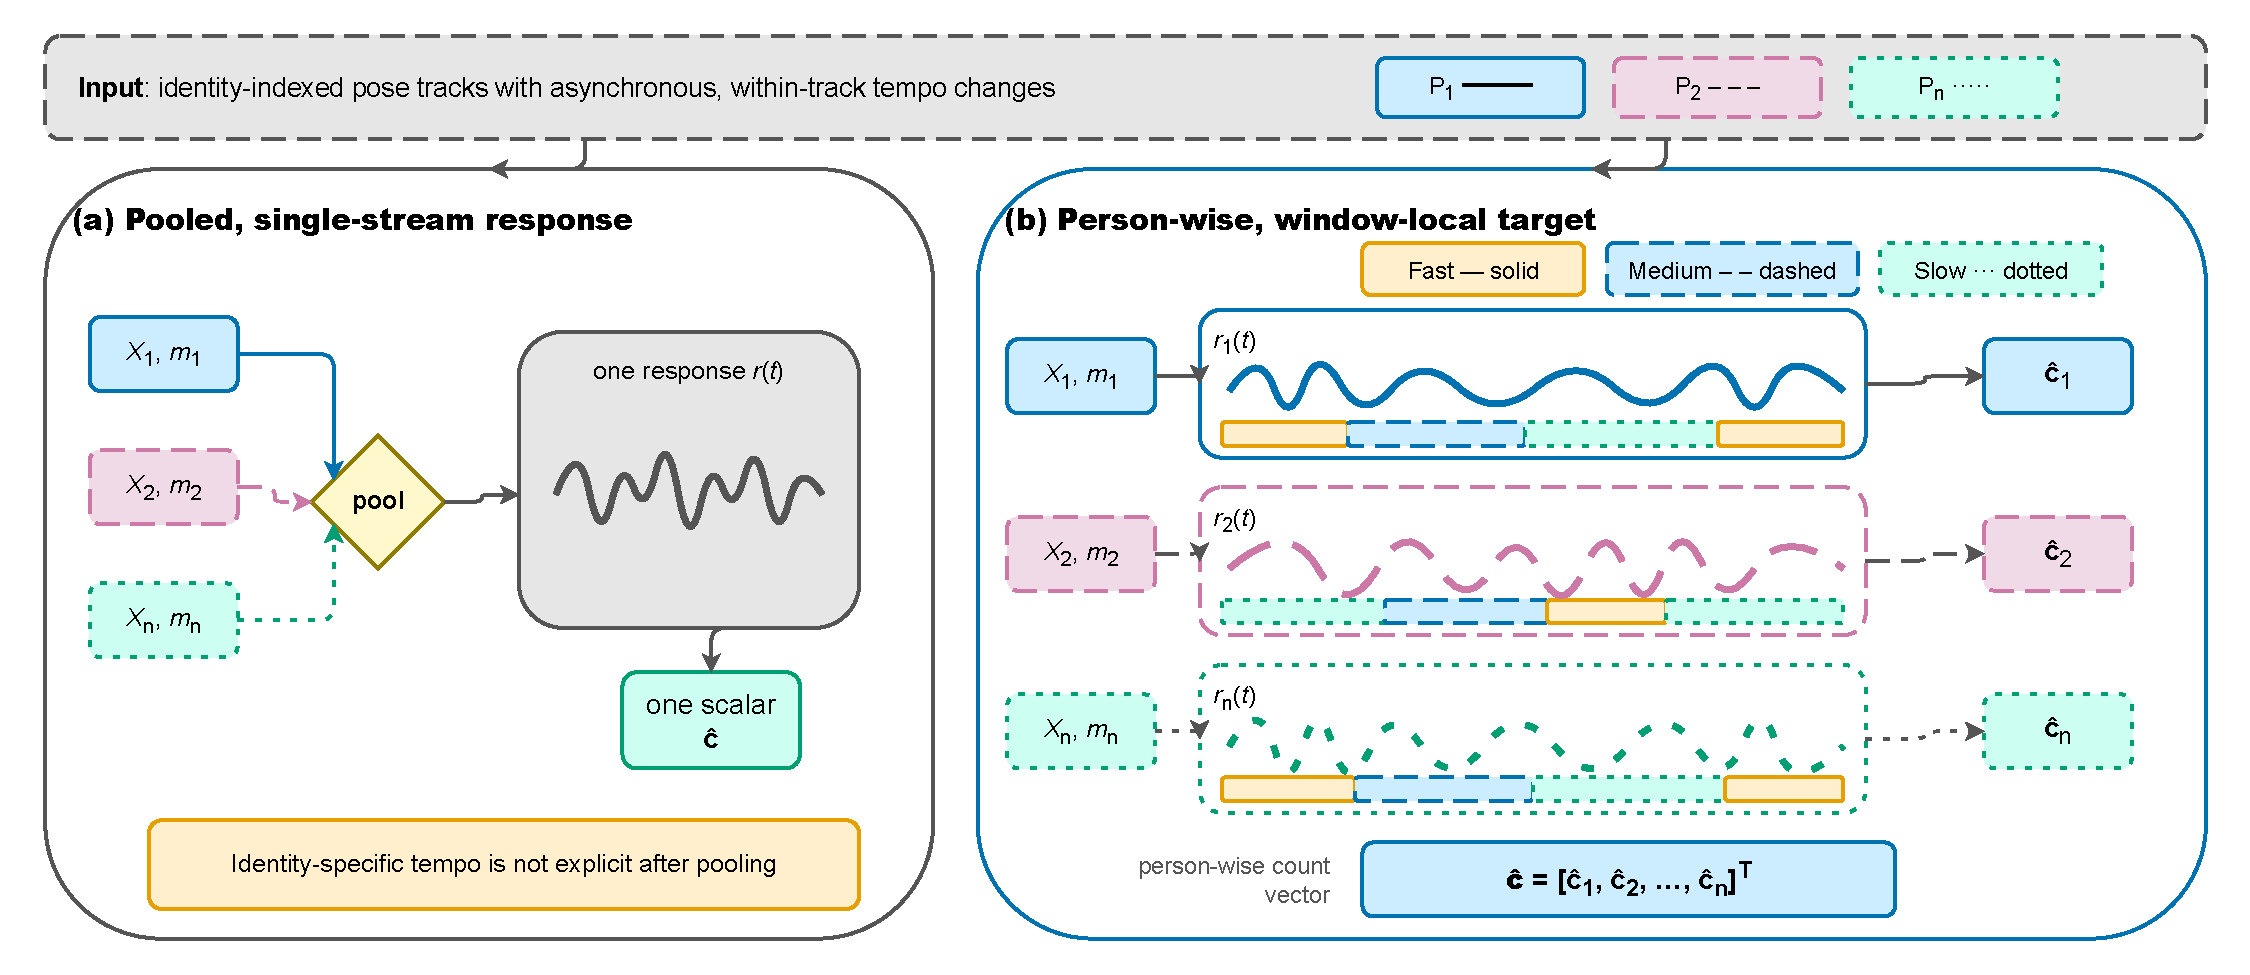
\includegraphics[width=0.98\textwidth]{figures/task_comparison.pdf}
  \caption{\textbf{Target task and output.} The left panel is a naïve pooled
  single-stream failure mode, not MultiCounter or MultiCounter+. A frame-level response can mix
  people who move at different and changing rates (left). We instead retain
  identity-indexed masked pose tracks, estimate tempo locally within each
  track, and return a person-wise count vector (right). The scene total is only
  a derived diagnostic. This is a problem illustration, not result evidence.}
  \label{fig:task_comparison}
\end{figure*}

The paper makes three falsifiable, currently evidence-gated contributions:

\begin{itemize}
  \item \ClaimMap{C01,C02}We formulate a pose-driven MRAC training setting whose intended
  counting loss uses no person-wise count or period annotations, while
  explicitly accounting for externally supervised perception components.
  This supervision statement must be verified against the frozen training
  graph before submission.

  \item \ClaimMap{C03,C04,C05,C06}We propose track-indexed, window-level tempo routing with
  shared parameters and per-track state, followed by response-domain
  overlap-add and one track-level decoding pass. Its benefit must be separated
  from the effects of tracking and the PAMS representation through controlled
  ablations.

  \item \ClaimMap{C10,C12,C15}We establish an evaluation contract that pairs the official MultiRep
  counting metrics with oracle/predicted-track protocols, tracking
  diagnostics, non-stationary-tempo stress tests, and person-count scaling.
  Every final table cell must be generated from a frozen result manifest.
\end{itemize}

This pre-results draft freezes the scientific story and its evidence
requirements; it does not assert that the multi-person modules are already
implemented or that the proposed method outperforms any baseline.

\section{Identity-Indexed Local Tempo Routing}
\label{sec:method}

The counter begins after perception: it receives pose trajectories with supplied
identity indices and validity masks. Oracle tracks, tracks from a frozen common
frontend, and native method pipelines define different experimental protocols
and are never ranked together. Parameters are shared, whereas buffers, periodic
evidence, masks, and responses remain identity-indexed; no window combines
people. Figure~\ref{fig:framework} summarizes the proposed specification, whose
tensor layouts and learned modules remain \SyncRequired{collaborator source
binding}. For predicted tracks, an index denotes a current tracklet, not a
guaranteed person. Fragmentation, re-entry, switches, retirement, and any
reconciliation belong to the \SyncRequired{track lifecycle contract}.

\begin{figure*}[t]
  \centering
  \TempoRACFrameworkGraphic
  \caption{Conceptual framework reproduced in full from the project's editable
  framework deck. In the manuscript, $M_i$ denotes an identity-indexed counter
  instance with shared learned parameters and separate state, not a separately
  parameterized model. The training strip lists candidate objectives: tempo
  routing and track-continuity terms remain \texttt{SYNC-REQUIRED} until they
  are bound to frozen code. PAMS-TCC is attributed to PAMS
  \cite{gao2026pams}. The diagram is not implementation or result evidence.}
  \label{fig:framework}
\end{figure*}

\subsection{Masked identity-indexed representation}
For person $i\in\{1,\ldots,N\}$, let \(\bX_i\) contain $J$ joints with $C$
coordinates over $T_i$ frames, and let $m_i(t)$ mark a valid observation.
Overlapping supports \(\cW_{i\ell}\) select local windows. A shared encoder
\(\cE_\theta\) maps the masked samples to features, while the primary output
remains a person-wise count vector:
\begin{equation}
\begin{aligned}
 \bX_i &\in \Rset^{T_i\times J\times C}\qquad
 m_i\in\Bset^{T_i}\qquad
 \widehat{\bc}=[\hat c_i]_{i=1}^{N} \\
 \bz_{i\ell}(t) &=
 \cE_\theta\!\left(\bX_i[\cW_{i\ell}]\mid m_i[\cW_{i\ell}]\right)_t
 \quad t\in\cW_{i\ell}
\end{aligned}
\label{eq:representation}
\end{equation}
\noindent Here $\Bset$ denotes the binary alphabet. The shared $\theta$ does
not mix identity state. Window geometry, pose
normalization, padding, short tracks, and buffer lifecycle are
\SyncRequired{track tensor and lifecycle contract}. Masks accompany every
transformation, and windows never cross identity timelines. A scene total
$\sum_i\hat c_i$ is diagnostic. Permutation, isolated-mask, and short-track
tests will check these invariants once the source interface exists.

\subsection{Local masked periodic evidence}
Tempo must vary with the window rather than being fixed for the whole track.
Let $s_{i\ell}(t)$ denote the scalar evidence signal provisionally projected
from \(\bz_{i\ell}(t)\), and $q_{i\ell}(t)$ its windowed validity mask. We
define a mask-normalized non-circular autocorrelation and a normalized Fourier
score, then map both to a period estimate and confidence:
\begin{equation}
\begin{aligned}
 \bar s_{i\ell} &=
 \frac{\sum_t q_{i\ell}(t)s_{i\ell}(t)}
      {\sum_t q_{i\ell}(t)+\epsilon} \\
 A_{i\ell}(\tau) &=
 \frac{\sum_t q_{i\ell}(t)q_{i\ell}(t+\tau)
 [s_{i\ell}(t)-\bar s_{i\ell}]
 [s_{i\ell}(t+\tau)-\bar s_{i\ell}]}
 {\sum_t q_{i\ell}(t)q_{i\ell}(t+\tau)+\epsilon} \\
 F_{i\ell}(\omega) &=
 \frac{\left|\sum_t q_{i\ell}(t)[s_{i\ell}(t)-\bar s_{i\ell}]
 e^{-\mathrm{j}\omega t}\right|^2}
 {\max_{\omega'}\left|\sum_t q_{i\ell}(t)[s_{i\ell}(t)-\bar s_{i\ell}]
 e^{-\mathrm{j}\omega' t}\right|^2+\epsilon} \\
 \begin{bmatrix}\hat p_{i\ell}\\\gamma_{i\ell}\end{bmatrix} &=
 \Phi\!\left(\{A_{i\ell}(\tau)\}_{\tau\in\cT}\mathbin\Vert
              \{F_{i\ell}(\omega)\}_{\omega\in\Omega}\right)
\end{aligned}
\label{eq:period}
\end{equation}
\noindent Indices $(i,\ell)$ expose within-track drift. Projection, centering,
domains and units, interpolation, confidence, and fallback are
\SyncRequired{period estimator}; Eq.~\ref{eq:period} fixes only the semantics of
local masked evidence. Confidence must measure available evidence rather than a
post-routing label, and low-support windows must be masked or use one frozen
fallback in training and evaluation. Since periodic visibility can induce
spectral peaks, the implementation must set out-of-range masks and minimum
lag-pair support and pass periodic/nonperiodic missingness controls. It must also
choose pair-dependent centering or another irregular-sample estimator
\cite{lomb1976unequal}.

\subsection{Soft routing over shared response experts}
Let \(\cK=\{\mathrm{fast},\mathrm{medium},\mathrm{slow}\}\) index shared
experts. A proposed router consumes the window representation, local period,
and confidence, and returns simplex weights. Each expert emits a continuous
local response rather than an independently rounded count:
\begin{equation}
\begin{aligned}
 \bu_{i\ell} &=
 \rho_\psi([\bz_{i\ell}\mathbin\Vert\hat p_{i\ell}\mathbin\Vert\gamma_{i\ell}]) \\
 \bg_{i\ell} &= \softmax(\bu_{i\ell}/\tau_{\mathrm r}) \\
 g_{i\ell k}&\geq0\qquad \sum_{k\in\cK}g_{i\ell k}=1 \\
 \br^{(k)}_{i\ell} &=
 \cH^{(k)}_{\phi_k}(\bz_{i\ell})\qquad k\in\cK
\end{aligned}
\label{eq:routing}
\end{equation}
\noindent Soft weights retain uncertainty at tempo transitions. Router inputs,
temperature, expert architecture, gradients, sharing, and fallback remain
\SyncRequired{router and expert implementation}. Fast/medium/slow are intended
scales, not observed specializations: paired controls must test expert use,
collapse, frozen tempo bands, and hard/uniform routing. Shared experts keep
parameter count independent of the number of tracks, but no runtime or memory
claim is enabled without profiling.

\subsection{Response reconstruction and one track decode}
The final stage mixes expert responses before merging overlapping windows. Let
$a_{i\ell}(t)$ be a taper on window \(\ell\), and let
$q_{i\ell}(t)$ exclude invalid samples. Normalized overlap-add forms a single
track response $R_i$, after which one decoder extracts events:
\begin{equation}
\begin{aligned}
 \widetilde{r}_{i\ell}(t) &=
 \sum_{k\in\cK}g_{i\ell k}r^{(k)}_{i\ell}(t) \\
 R_i(t) &=
 \frac{\sum_{\substack{\ell\\t\in\cW_{i\ell}}}
 a_{i\ell}(t)q_{i\ell}(t)\widetilde{r}_{i\ell}(t)}
 {\sum_{\substack{\ell\\t\in\cW_{i\ell}}}
 a_{i\ell}(t)q_{i\ell}(t)+\epsilon} \\
 \widehat{\cE}_i &= \cD(R_i\mid m_i)\qquad
 \hat c_i=|\widehat{\cE}_i|
\end{aligned}
\label{eq:reconstruction}
\end{equation}
\noindent This order avoids counting every window independently; it does not
guarantee one peak. Decoded samples require aligned timestamps and coverage
$\sum_\ell a_{i\ell}(t)q_{i\ell}(t)>0$. Taper, gaps, event confidence, peak
parameters, and decoder semantics remain \SyncRequired{reconstruction and
decoder}. PAMS-TCC is the documented starting objective \cite{gao2026pams};
$\cL_{\mathrm{PAMS\text{-}TCC}}+\lambda_{\mathrm r}\cL_{\mathrm{route}}
+\lambda_{\mathrm t}\cL_{\mathrm{track}}$ is only a synchronization contract.
The latter terms, their existence, formulas, weights, samples, supervision, and
gradient paths must bind to code; absent terms will be deleted. Overlap-add
preserves continuous evidence before one masked trajectory-level decode. A
boundary test will place an event at several offsets and test one-time decoding.

The supervision audit must inspect loaders, pseudo-targets, auxiliary losses,
selection, stopping, calibration, and inference fallbacks at one commit. Until
it passes, the paper states only the intended absence of person-wise count and
period labels in the counting objective and discloses perception supervision.

% Encounter the paired table float before the experiments text so that the
% two panels can occupy the top of technical page four rather than page five.
\begin{table*}[!t]
\centering
\begin{minipage}[t]{0.625\textwidth}
\centering
\caption{Protocol-separated main comparison. Arrows indicate metric direction;
pending cells contain no measurement.}
\label{tab:main}
\setlength{\tabcolsep}{1.35pt}
\tiny
\begin{tabular}{llccccc}
\toprule
Method & Protocol & P-mAP $\uparrow$ & AP50 $\uparrow$ & AP75 $\uparrow$ & MAE $\downarrow$ & OBO $\uparrow$ \\
\midrule
MultiCounter \cite{tang2024multicounter} & native & \pendingcell{mc-pmap} & \pendingcell{mc-ap50} & \pendingcell{mc-ap75} & \pendingcell{mc-mae} & \pendingcell{mc-obo} \\
MultiCounter+ \cite{tang2026multicounterplus} & native & \pendingcell{mcp-pmap} & \pendingcell{mcp-ap50} & \pendingcell{mcp-ap75} & \pendingcell{mcp-mae} & \pendingcell{mcp-obo} \\
\midrule
Track-PAMS \cite{gao2026pams} & oracle & \pendingcell{otp-pmap} & \pendingcell{otp-ap50} & \pendingcell{otp-ap75} & \pendingcell{otp-mae} & \pendingcell{otp-obo} \\
Global tempo & oracle & \pendingcell{otg-pmap} & \pendingcell{otg-ap50} & \pendingcell{otg-ap75} & \pendingcell{otg-mae} & \pendingcell{otg-obo} \\
TempoRAC & oracle & \pendingcell{oours-pmap} & \pendingcell{oours-ap50} & \pendingcell{oours-ap75} & \pendingcell{oours-mae} & \pendingcell{oours-obo} \\
\midrule
Track-PAMS \cite{gao2026pams} & common track & \pendingcell{tp-pmap} & \pendingcell{tp-ap50} & \pendingcell{tp-ap75} & \pendingcell{tp-mae} & \pendingcell{tp-obo} \\
Global tempo & common track & \pendingcell{tg-pmap} & \pendingcell{tg-ap50} & \pendingcell{tg-ap75} & \pendingcell{tg-mae} & \pendingcell{tg-obo} \\
TempoRAC & common track & \pendingcell{ours-pmap} & \pendingcell{ours-ap50} & \pendingcell{ours-ap75} & \pendingcell{ours-mae} & \pendingcell{ours-obo} \\
\bottomrule
\end{tabular}
\end{minipage}\hfill
\begin{minipage}[t]{0.355\textwidth}
\centering
\caption{Paired mechanism ablations. Deltas are variant minus the soft-routing
NOLA reference.}
\label{tab:ablation}
\setlength{\tabcolsep}{1.25pt}
\tiny
\begin{tabular}{llllcc}
\toprule
Tempo & Cue & Route & Merge & $\Delta$MAE & $\Delta$OBO \\
\midrule
global & A+F & uniform & NOLA & \pendingcell{abl-global-mae} & \pendingcell{abl-global-obo} \\
local & ACF & soft & NOLA & \pendingcell{abl-acf-mae} & \pendingcell{abl-acf-obo} \\
local & FFT & soft & NOLA & \pendingcell{abl-fft-mae} & \pendingcell{abl-fft-obo} \\
local & A+F & single & NOLA & \pendingcell{abl-single-mae} & \pendingcell{abl-single-obo} \\
local & A+F & hard & NOLA & \pendingcell{abl-hard-mae} & \pendingcell{abl-hard-obo} \\
local & A+F & soft & boxcar & \pendingcell{abl-boundary-mae} & \pendingcell{abl-boundary-obo} \\
local & A+F & soft & window & \pendingcell{abl-window-mae} & \pendingcell{abl-window-obo} \\
local & A+F & soft & NOLA & 0 & 0 \\
\bottomrule
\end{tabular}
\end{minipage}
\end{table*}

\section{Experiments}
\label{sec:experiments}

\paragraph{Pre-results status.}
This section fixes the evaluation questions, protocols, and table schemas; it
contains no new-method measurement or empirical conclusion. Red entries are
controlled evidence fields. Historical UCFRep dev84 diagnostics, proxy
readouts, and runs involving an untrained random Period Head are ineligible for
every table below.

\subsection{Evaluation Contract}
\label{sec:evaluation_contract}
\ClaimMap{C07,C10,C11,C12,C15}

\paragraph{Data and integrity.}
The primary benchmark will be the exact MultiRep release
\Protocol{multirep.release} under its official \Protocol{multirep.split}
protocol. The original MultiCounter paper specifies 1,157 synthetic videos,
52,590 periodic events, and a 7:2:1 train/validation/test split, while the
current MultiCounter+ repository reports the same size and provides a download
without a versioned release identifier or checksums
~\cite{tang2024multicounter,tang2026multicounterplus}. The final manifest must
therefore bind the release identifier, download source and time,
video/annotation/split SHA-256 digests, evaluator revision, and preprocessing
fingerprint. A run is table-ineligible if any binding is missing or if
incompatible artifacts are mixed. Before model comparison, a frozen dataset
characterization report must give split-level counts of videos, ground-truth
people, events, active-person levels, within-track tempo dispersion, detected
accelerations/decelerations, pauses, observation gaps, and identities with
enough cycles for every declared window length. Stratum definitions and counts
are fixed before looking at method errors.

\paragraph{Oracle and predicted tracks.}
The oracle-track protocol supplies official person identities and spatial
support, isolating repetition counting from detection and association. The
predicted-track protocol uses one frozen detector--pose--tracker frontend for
all compatible track-conditioned counters. Native joint MRAC systems retain
their audited official pipelines and appear in a separate contextual block,
not as if their inputs were controlled. Against ground-truth identities and
spatial support, HOTA and its DetA, AssA, and LocA components
~\cite{luiten2021hota} diagnose predicted-track detection, association, and
localization quality. IDF1 and ID-switch counts~\cite{ristani2016idmetrics}
provide complementary identity-duration and temporal-association diagnostics.
When the same frozen tracks feed several counters, these tracking values must
be identical and cannot be credited as counting gains.

\paragraph{Evaluator-ready outputs.}
Each counter adapter must emit the scored event tuples in
Equation~\ref{eq:event_schema}, the raw per-track count vector, and the exact
spatial support expected by the pinned evaluator. Oracle tracks retain official
identity support. Predicted tracks remain separate through evaluation: the
manifest-bound adapter must specify one deterministic matching policy and how
unmatched, duplicated, fragmented, merged, and identity-switched tracks become
false positives or false negatives. No post-hoc fragment joining is allowed
unless it is a separately audited method component. Adapter source, tests, and
per-instance outputs are required before Period-mAP or matched person-wise
count metrics become table-eligible. Predicted-track outputs are called
track-wise until this matching is applied.

\paragraph{Metrics and uncertainty.}
Using the frozen official evaluator, we will report Period-mAP, AP50, AP75,
AvgMAE, and AvgOBO, together with a matched person-count error
diagnostic after the evaluator's frozen matching step. Period-mAP under common
predicted tracks is the confirmatory metric; the primary contrast is our method
minus track-conditioned PAMS on identical videos and frontend outputs. A claim
of improvement requires the lower endpoint of its paired 95\% interval to be
above zero. Native-pipeline rows are descriptive and cannot establish
non-inferiority or superiority under a common-input protocol.

Every reproducible method uses at least three pre-registered seeds, reported
as mean and between-seed sample standard deviation. The confirmatory interval
uses one pre-declared paired hierarchical bootstrap: each replicate resamples
completed seed pairs and then videos within each sampled seed, retaining every
identity of a sampled video and recomputing Period-mAP from event records rather
than averaging per-video AP. Its point estimate is the mean of paired
seed-level differences. The manifest fixes the resample count, random seed,
failed-run policy, and exact numbers of completed seeds, videos, people, and
events. Secondary ablations are exploratory, with family-wise Holm correction
if formal significance statements are made. Official
single-checkpoint numbers remain explicitly marked and are excluded from
variance and significance claims. Test annotations are not used for tuning,
checkpoint selection, routing calibration, or early stopping.

The numerical stabilizer \(\epsilon\) is fixed before evaluation in the units
of each denominator. A sensitivity check spans representable smaller and larger
values and reports changes in response amplitude and count metrics by valid
support; it must expose, rather than hide, any coverage dependence introduced
by Equations~\ref{eq:valid_mean} and~\ref{eq:normalized_ola}.

\paragraph{Baselines and supervision.}
The mandatory native baselines are MultiCounter and MultiCounter+
~\cite{tang2024multicounter,tang2026multicounterplus}. Under the common track
interface we adapt RepNet~\cite{dwibedi2020repnet},
TransRAC~\cite{hu2022transrac}, PoseRAC~\cite{yao2025poserac}, and
PAMS~\cite{gao2026pams}; DeTRC~\cite{ma2026detrc} and
D$^2$-STX~\cite{wang2026d2stx} are candidate baselines and enter only if
runnable public implementations are available and their output semantics
pass the experiment audit. Tables disclose input modality, training labels,
track source, run count, adapter code, crop/pose construction, training split,
tuning budget, pretrained checkpoint, and output conversion. Comparisons across supervision regimes are
accuracy--annotation trade-offs, not claims of identical training information.

\subsection{Primary Questions}
\label{sec:primary_questions}
\ClaimMap{C03,C04,C05,C06,C12,C15}

The evaluation is organized around four questions. First, how does a
no-count-label pose counter compare on person-wise oracle-track MRAC and on
matched predicted tracks? Second, does local routing help beyond a track-conditioned
PAMS base when tempo changes within one identity? Third, does response-domain
overlap-add reduce boundary errors relative to summing independently decoded
windows? Fourth, how do tracking errors, active-person count, and upstream
preprocessing affect robustness and efficiency? Each question has a named
table or figure and an associated claim that remains withheld until the
evidence audit passes. The mechanism study must also compare against running
PAMS independently per track, sliding-window PAMS without a learned router,
deterministic tempo bins, non-overlapping and center-crop decoding, uniform
response averaging, and phase-aligned fusion.

\begin{table*}[t]
  \centering
  \small
  \setlength{\tabcolsep}{3.1pt}
  \caption{Planned MultiRep main results. Reproducible rows will show the
  mean and sample standard deviation over pre-registered seeds; official
  single-checkpoint rows will be marked. Protocol blocks answer different
  questions and will not be pooled into one ranking.}
  \label{tab:main_multirep}
  \begin{tabular}{lllccccc}
    \toprule
    Method & Track protocol & Count supervision &
    Period-mAP$\uparrow$ & AP50$\uparrow$ & AP75$\uparrow$ &
    AvgMAE$\downarrow$ & AvgOBO$\uparrow$ \\
    \midrule
    \multicolumn{8}{l}{\textit{Controlled oracle tracks}}\\
    RepNet & Oracle & \Protocol{sup.repnet} & \R{main.oracle.repnet.pmap} &
      \R{main.oracle.repnet.ap50} & \R{main.oracle.repnet.ap75} &
      \R{main.oracle.repnet.mae} & \R{main.oracle.repnet.obo} \\
    TransRAC & Oracle & \Protocol{sup.transrac} &
      \R{main.oracle.transrac.pmap} & \R{main.oracle.transrac.ap50} &
      \R{main.oracle.transrac.ap75} & \R{main.oracle.transrac.mae} &
      \R{main.oracle.transrac.obo} \\
    PoseRAC & Oracle & \Protocol{sup.poserac} & \R{main.oracle.poserac.pmap} &
      \R{main.oracle.poserac.ap50} & \R{main.oracle.poserac.ap75} &
      \R{main.oracle.poserac.mae} & \R{main.oracle.poserac.obo} \\
    PAMS & Oracle & \Protocol{sup.pams} & \R{main.oracle.pams.pmap} &
      \R{main.oracle.pams.ap50} & \R{main.oracle.pams.ap75} &
      \R{main.oracle.pams.mae} & \R{main.oracle.pams.obo} \\
    \textbf{Ours} & Oracle & \Protocol{sup.ours} & \R{main.oracle.ours.pmap} &
      \R{main.oracle.ours.ap50} & \R{main.oracle.ours.ap75} &
      \R{main.oracle.ours.mae} & \R{main.oracle.ours.obo} \\
    \midrule
    \multicolumn{8}{l}{\textit{Controlled common predicted tracks}}\\
    RepNet & Common predicted & \Protocol{sup.repnet} &
      \R{main.pred.repnet.pmap} & \R{main.pred.repnet.ap50} &
      \R{main.pred.repnet.ap75} & \R{main.pred.repnet.mae} &
      \R{main.pred.repnet.obo} \\
    TransRAC & Common predicted & \Protocol{sup.transrac} &
      \R{main.pred.transrac.pmap} & \R{main.pred.transrac.ap50} &
      \R{main.pred.transrac.ap75} & \R{main.pred.transrac.mae} &
      \R{main.pred.transrac.obo} \\
    PoseRAC & Common predicted & \Protocol{sup.poserac} &
      \R{main.pred.poserac.pmap} & \R{main.pred.poserac.ap50} &
      \R{main.pred.poserac.ap75} & \R{main.pred.poserac.mae} &
      \R{main.pred.poserac.obo} \\
    PAMS & Common predicted & \Protocol{sup.pams} & \R{main.pred.pams.pmap} &
      \R{main.pred.pams.ap50} & \R{main.pred.pams.ap75} &
      \R{main.pred.pams.mae} & \R{main.pred.pams.obo} \\
    \textbf{Ours} & Common predicted & \Protocol{sup.ours} & \R{main.pred.ours.pmap} &
      \R{main.pred.ours.ap50} & \R{main.pred.ours.ap75} &
      \R{main.pred.ours.mae} & \R{main.pred.ours.obo} \\
    \midrule
    \multicolumn{8}{l}{\textit{Native full-pipeline context; descriptive only}}\\
    MultiCounter & Native & \Protocol{sup.multicounter} &
      \R{main.native.multicounter.pmap} & \R{main.native.multicounter.ap50} &
      \R{main.native.multicounter.ap75} & \R{main.native.multicounter.mae} &
      \R{main.native.multicounter.obo} \\
    MultiCounter+ & Native & \Protocol{sup.multicounterplus} &
      \R{main.native.multicounterplus.pmap} &
      \R{main.native.multicounterplus.ap50} &
      \R{main.native.multicounterplus.ap75} &
      \R{main.native.multicounterplus.mae} &
      \R{main.native.multicounterplus.obo} \\
    \bottomrule
  \end{tabular}
\end{table*}

The quantitative interpretation of Table~\ref{tab:main_multirep} remains
withheld until every displayed binding passes the empirical audits.

\begin{table*}[t]
  \centering
  \small
  \setlength{\tabcolsep}{3.0pt}
  \caption{Required protocol disclosure accompanying the main table. Native
  rows retain their official pipelines and are not pooled with common-input
  rows. Every field is manifest-bound.}
  \label{tab:protocol_disclosure}
  \begin{tabular}{lllllll}
    \toprule
    Method & Result block & Input & Count labels & Period labels & Track source & Runs \\
    \midrule
    RepNet & Common & \Protocol{disc.repnet.input} & \Protocol{disc.repnet.count} &
      \Protocol{disc.repnet.period} & \Protocol{disc.common.track} & \Protocol{disc.repnet.runs} \\
    TransRAC & Common & \Protocol{disc.transrac.input} & \Protocol{disc.transrac.count} &
      \Protocol{disc.transrac.period} & \Protocol{disc.common.track} & \Protocol{disc.transrac.runs} \\
    PoseRAC & Common & \Protocol{disc.poserac.input} & \Protocol{disc.poserac.count} &
      \Protocol{disc.poserac.period} & \Protocol{disc.common.track} & \Protocol{disc.poserac.runs} \\
    PAMS & Common & \Protocol{disc.pams.input} & \Protocol{disc.pams.count} &
      \Protocol{disc.pams.period} & \Protocol{disc.common.track} & \Protocol{disc.pams.runs} \\
    \textbf{Ours} & Common & \Protocol{disc.ours.input} & \Protocol{disc.ours.count} &
      \Protocol{disc.ours.period} & \Protocol{disc.common.track} & \Protocol{disc.ours.runs} \\
    MultiCounter & Native context & \Protocol{disc.multicounter.input} &
      \Protocol{disc.multicounter.count} & \Protocol{disc.multicounter.period} &
      \Protocol{disc.multicounter.track} & \Protocol{disc.multicounter.runs} \\
    MultiCounter+ & Native context & \Protocol{disc.multicounterplus.input} &
      \Protocol{disc.multicounterplus.count} & \Protocol{disc.multicounterplus.period} &
      \Protocol{disc.multicounterplus.track} & \Protocol{disc.multicounterplus.runs} \\
    \bottomrule
  \end{tabular}
\end{table*}

\begin{table}[t]
  \centering
  \small
  \setlength{\tabcolsep}{2.7pt}
  \caption{Planned construction-path diagnostic under oracle tracks. LT: local
  tempo; SR: soft routing; BS: boundary stitching; TC: track-continuity
  objective. Causal conclusions use removals from the full model and the
  factorial controls described below, not this order-dependent path alone.}
  \label{tab:additive_ablation}
  \begin{tabular}{lcccccc}
    \toprule
    Variant & LT & SR & BS & TC & Period-mAP$\uparrow$ & AvgMAE$\downarrow$ \\
    \midrule
    Track-PAMS & & & & & \R{abl.base.pmap} & \R{abl.base.mae} \\
    $+$ LT & \checkmarkcell & & & & \R{abl.lt.pmap} & \R{abl.lt.mae} \\
    $+$ SR & \checkmarkcell & \checkmarkcell & & &
      \R{abl.sr.pmap} & \R{abl.sr.mae} \\
    $+$ BS & \checkmarkcell & \checkmarkcell & \checkmarkcell & &
      \R{abl.bs.pmap} & \R{abl.bs.mae} \\
    $+$ TC & \checkmarkcell & \checkmarkcell & \checkmarkcell &
      \checkmarkcell & \R{abl.tc.pmap} & \R{abl.tc.mae} \\
    \bottomrule
  \end{tabular}
\end{table}

The ablation interpretation remains withheld until all rows share one frozen
protocol and have the required paired records. The full mechanism study also
removes each component one at a time, crosses local-tempo estimation, routing,
and stitching in a small factorial design, matches single- and multi-expert
capacity, tests experts with and without direct \(\hat p\), and reports route
occupancy, entropy, collapse, and specialization by tempo stratum.

The appendix pre-registers router variants, expert counts, local-versus-global
tempo, shared batched execution versus independent same-checkpoint replicas,
boundary and continuity ablations,
tempo/occlusion/identity-switch stress, cross-dataset transfer, and latency,
memory, FLOPs, and throughput as the number of active identities grows. All
plots and tables must be generated from frozen JSON, CSV, or Parquet records;
manually transcribed values are inadmissible.

\section{Conclusion and Limitations}
\label{sec:conclusion}

We specify a pose-driven MRAC counter for people whose pace changes within a
track. The central design separates identity state while sharing parameters,
routes overlapping windows from local period evidence, fuses continuous
responses by normalized overlap-add, and decodes each track once. The setting
does not remove all annotation and does not jointly optimize perception and
counting: the counting objective is intended to avoid person-wise count and
period labels, while upstream perception may use external supervision.

This draft has three material limitations. The current local checkout contains
only a single-person PAMS reproduction; the multi-person data path, router,
continuity loss, and boundary decoder await synchronization with collaborator
code. No eligible MultiRep artifact has been received, so the manuscript makes
no performance claim. Finally, a modular pose/track pipeline inherits missed
detections and identity switches and may scale with the number of active
people. The final study must quantify each limitation through oracle/predicted
tracks, corruption analysis, and population-scaling measurements. Until those
gates close, the paper remains provisional and data-pending. MultiRep is
synthetic, and single-person transfer cannot establish multi-person identity
preservation; absent a real multi-person evaluation, any eventual conclusion
must remain restricted to MultiRep and the declared controlled tracker
corruptions.


% The live ICASSP 2027 rule restricts the optional fifth page to references.
% These declarations therefore remain inside the four-page body.
\noindent\textbf{Funding, conflicts of interest, and ethical compliance.}
Funding and conflict-of-interest declarations are \Pending{author-declarations}.
The final ethical-compliance statement is \Pending{ethical-compliance} and will
be bound to the dataset licenses, participant provenance, and release terms
before submission.

{\small
\bibliographystyle{vendor/icassp2026/IEEEbib}
\bibliography{references}
}

\end{document}
